
\Chapter{
    ``For you are dust, and to dust shall you return.''
\\[5pt]
\rightline{{\rm --- The book of genesis 3:19}}
}{The Roles and Physics of Aeolian Dust}
The first part of this chapter provides the necessary context and prerequisite knowledge on the roles of aeolian dust in the climate system, the importance of dust as a record of environmental change and the physics behind dust modelling. In the second and last part of this chapter, the scope is narrowed down to the East Asian region. It will begin by describing the location and characteristics of the main source and dust fallout regions, followed by an overview of the meteorological conditions responsible for producing dust events and their climatology. 

\section{Dust's role in the climate system}\label{seq:physics_of_dust}

\begin{figure}[htpb]
    \centering
    \includegraphics[width=\textwidth]{texfiles/figs/Desert_distrubtion.PNG}
    \caption{Earth's distribution of arid regions, adopted from \textcite{williams_climate_2014}}
    \label{fig:desert_distrubtion}
\end{figure}
Aeolian dust is one of the most abundant aerosol species in the atmosphere and accounts for most of the total atmospheric aerosol mass. Aeolian dust refers to dust that is emitted and transported by winds, and the word aeolian stems from the Greek god Aeolus, which in Greek mythology is the keeper of the winds. Around 1/3 of the earth surface is covered by deserts, that is, regions where the precipitation is too low and evaporation too high to allow plants to grow \parencite{williams_climate_2014}.
As shown in \Cref{fig:desert_distrubtion} a large portion of the arid regions are located between 20\degree - 40\degree north/south. This region is known as the dust belt. The dust belt coincides with the descending part of the Hadley circulation, where the descending motion increases the atmosphere's stability and suppress the formation of rainfall. 
Other areas that typically experience a minimal amount of rainfall are places situated in the rain shadow of the surrounding topography or far in the interior of the continents where there are no proximal sources of moisture.  
The main dust sources are found in regions such as the Sahara, Middle East and northwest China. 

The dry conditions produce loose soils that are easily erodible. Thus during periods of strong winds, dust emissions are naturally produced and entrained into the atmosphere. 
The world's deserts produce an estimated 2000Mt of atmospheric dust globally each year, with around 1500Mt being deposited on land and about 500Mt being deposited into the ocean \parencite{shao2011dust}. 
If the dust gets entrained into the upper troposphere, it can be transported by the winds for thousands of kilometres \parencite{yumimoto_elevated_2009}. In the atmosphere, the dust particles directly affect the transfer of radiation through the atmosphere. 
The smallest dust particles between 0.2-\SI{2}{\micro\metre} have a size around the same order as the wavelength of visible light and are the most efficient at scattering incoming solar radiation back to space. Accordingly, the smallest particles have a cooling effect on climate. Conversely, the larger particles (> \SI{4}{\micro\metre}) produces has a warming effect on climate due to their larger size, which makes them efficient at absorbing terrestrial longwave radiation \parencite{choobari2014global}.
The lifetime of the dust aerosols is also strongly dependent on particle size \parencite{mahowald2014size}. Constraining the direct radiative effect of dust aerosols requires thus both getting the magnitude and size distribution of the emitted dust correct \parencite{adebiyi2020dust}.

In the atmosphere, dust also interacts with clouds by acting as \acrfull{in} and \acrfull{ccn} altering the microphysical properties of the clouds \parencite{lohmann2006sensitivity}. Dust aerosols in their unaltered state are usually hydrophobic and thus quite inefficient \acrshort{ccn}. However, during transport, dust aerosols can acquire a coating of soluble material, enhancing their ability to act as \acrshort{ccn} \parencite{Dust_aerosols_coating2001}. Dust aerosols have also been suggested to warm the clouds as dusty clouds have been observed to have a lower liquid water path compared to their dust-free counterparts, through the aerosol semi-direct effect \parencite{huang2006satellite}. The semi-direct effect might play a significant role in inhibiting precipitation over the desert regions, reinforcing the aridity of the desert \parencite{shao2011dust}.  However, there are large uncertainties in the radiative impact of dust aerosols on clouds due to how sensitive clouds are to even small changes in their microphysical properties (e.g. droplet size, droplet concentration and cloud phase).
%Dust aerosols have also been discovered to influence tropical cyclones. Where tropical cyclones that have been seen to intercept dust clouds was found to be significantly weaker after passing through the dust cloud. The increase in \acrshort{ccn} caused by the dust plume slowed the rate of converting cloud drops into precipitation, affecting the amount and distribution of latent heat \parencite{rosenfeld2011pollution}.  

Beyond the time dust reside in the atmosphere, dust deposition also has a large impact on climate through influencing ecosystems and changing the snow surface albedo \parencite{shao2011dust} \todo{one more citation}. 
In particular, ocean biomass productivity is dependent on dust as a source of iron. In the ocean, iron is a limiting factor for phytoplankton production, which is responsible for nearly half of the annual \ch{CO2} exchange between the atmosphere and the ocean and the majority of carbon sequestration on geological time scales \parencite{shao2011dust}. Moreover, the impact of dust is not limited to ocean productivity. African dust is an important source of nutrients for the Amazon rainforest \todo{citation}. The productivity of the Amazon rainforest is constrained by the availability of phosphorus. \textcite{yu2015fertilizing} estimated about 0.022 Tg of phosphorus is brought to the Amazon through deposition of Sharan dust each year, comparable to the amount washed out by rainfall. Model estimates of dust variability during the 20th century showed that increased dust deposition to the ocean and the corresponding boost of ocean productivity has caused an additional 4ppm of \ch{CO2} to be taken up by the ocean. However, regional shifts in precipitation and temperature due to desert dust changes caused a similar decrease of 6ppm \ch{CO2} in the terrestrial biosphere carbon sink \parencite{mahowald2010observed}. Demonstrating that determining the net influence of dust on the biosphere and the carbon cycle is not straightforward.
\subsection{Dust as a Climate Archive}
Dust emission fluxes, size distribution and mineralogical composition are all strongly influenced by the wind speed, soil moisture and vegetation cover, and therefore indirectly modulating the influence of dust in the climate system. 
These climatic variables have experienced large changes throughout the history of Earth's climate and, more pressingly, are expected to change under the ongoing human caused global warming. Dust transport is affected by changes in the atmospheric circulation and wet deposition by precipitation changes. There is, consequently,
a potential for feedbacks involving dust and climate change. Thus dust archives are a window into the past from which the interconnections between climate and dust can be studied and provide insight on how the role dust might change in the near future climate. 

Arguably the most important dust record is the Loess record. Loess consists of aeolian sediments and are typically dominated by silt-sized (2-\SI{50}{\micro\metre}) particles \parencite{muhs2014loess}. Terrestrial loess occupies large areas of North America, China, Central Asia and Europe, with the most prominent Loess deposits located at the \acrfull{clp}.
Variations in \acrfull{mar}, particle size distribution have been used to reconstruct changes in large scale-circulation patterns and dust transport pathways, climatic changes in the dust source and deposition areas, and provide constraints for model reconstructions of past global climate states\todo{reference}. In addition to loess, aeolian dust is also found in ice cores and deep-sea records. One of the best-documented features in the dust record is the variation in \acrfull{mar} between the glacial and interglacial periods. During glacial stages, the earth experienced increased dust loading. Findings from the dust records suggest that during the glacial periods the high latitude dust loading were up to 25 times the present value and around two times at the lower latitude \parencite{shao2011dust}.     


\section{Dust Modelling}\label{sec:dust_modelling}
The important role of dust in the climate system, as pointed out in the previous section, has inspired researchers across the scientific disciplines to put considerable efforts towards developing global and regional dust models. 
The field of dust modelling started to take off in the early 1990s when scientists realised that aerosols, including dust, were responsible for a large fraction of the uncertainties in the climate models due to the difficulties in determining the aerosol radiative effect \parencite{tegen1996influence}, as described in \Cref{seq:physics_of_dust}. 
Models have improved since then, and current state of the art models can reproduce large scale patterns of atmospheric dust load \todo{citation}. 
However, uncertainties in the description of source areas and processes controlling dust emission and deposition produce a large spread in simulated dust fluxes \parencite{huneeus2011global}. 
This section provides an overview of the parameterisations of dust emissions, transport and deposition processes used in current dust models. 
%The last part of this chapter will discuss some of the main discrepancies and uncertainties of current dust models.
 
\subsection{Dust Emissions}\label{sec:dust_emission_modelling}
Producing a realistic estimate of the spatial distribution of dust emission flux depends on the model realistically representing surface properties and surface winds. Moreover, dust emissions are highly variable both spatially and temporally, which means that the dust model has to account for emissions that occur on scales that are not explicitly resolved in the model.        

Dust is mobilised when the force exerted by the wind on the bare soil exceed the mobilisation threshold. The forces acting on a dust particle at rest are the aerodynamic force that exerts lift and gravitational and interparticle forces that tend to fix the particle in place. 
The strength aerodynamic force is governed by the amount of momentum transferred from the atmosphere to the surface, described in terms of a friction velocity $u^*$ \parencite{ShaoYaping2008PaMo}.
\begin{equation}
    u_* = \sqrt{\tau/\rho}
\end{equation}
Here $\tau$ is the vertical component of the momentum flux, and $\rho$ is the air density. The strength of the forces counteracting dust mobilisation primarily depends on the particle size. The effect of the interparticle forces decreases with larger particle size, but the larger particles are also heavier and therefore feel a stronger tug by gravity. Thus the particles most easily mobilised by the wind have a size corresponding to where the interparticle and gravitational forces are approximately equal in magnitude.     
The amount of force the wind has to exert on the dust particle to exceed the forces counteracting mobilisation is expressed by the threshold friction velocity. The expression obtained by \textcite{shao2000simple} is often used in the dust modelling community as it is relatively straightforward. 
\begin{equation}\label{eq:treshold_fric_vel}
    u_{*t0}(d) = \sqrt{a_1 \left(\frac{\rho_p}{\rho_a}gd+\frac{a_2}{\rho_ad}\right)} 
\end{equation}
Here $a_1$ is a tuning parameter, $a_2$ is the scaling constant for the inter particle forces, $\rho_p$ is the particle density and $\rho_a$ is the air density. \textcite{shao2000simple} achieved good agreement with observations for $a_1 = 3.0\si{\kg\per\s\squared}$ and $a_2 = 0.0123$. 
The balance between the $u^*$ and $u^*_t$ is sensitive to environmental factors such as weather (e.g. wind, precipitation and temperature), the soil composition, the soil moisture content, soil particle size distribution, vegetation converge and topography \todo{citation}.  
\textbf{\begin{figure}[hptb]
    \centering
    \includegraphics[scale=0.7]{../figs/Threshold_friction_velocity.PNG}
    \caption{Threshold friction velocity $\mathbf{u^*}$ as a function of particle diameter. Points represent measurements from wind tunnel experiments, and the lines represent different semi-empirical expressions for the threshold friction velocity \parencite{kok2012physics}}.
    \label{fig:treshold_friction_velocity_ps}
\end{figure}}  
All these factors vary significantly both spatially and temporally, making accurately calculating the threshold friction velocity difficult \todo{reference}. \Cref{fig:treshold_friction_velocity_ps} show the the threshold friction velocity as a function of particle diameter, the coloured lines represent the semi-empirical relations for $u^*_t$ described in \textcite{iversen1982saltation} (pink), \textcite{shao2000simple} (green) and \textcite{bagnold1941physics}. The semi-empirical relations and measurement seems to agree on a minimum in $u^*_t$ around in the range between  \SI{75}{\micro\metre} - \SI{100}{\micro\metre}. However, these particles are too heavy to be subject to long-range suspension and will soon after entrainment take on ballistic trajectories.
The impact from the large particle hitting the soil bed then eject smaller dust particles (\SI{20}{\micro\metre} < ) and 
these smaller particles can be subjected to long-range transport. This process is known as sandblasting is the predominant process causing dust emissions, and in dust models, minor processes are often neglected. 

There have been proposed several physics-based schemes for estimating the vertical dust \parencite{MB95_dust_emission,alfaro2001modeling,shao2004simplification}. The main distinction between the present schemes lay in how the particle size information is represented in the model. The schemes can be divided into one of two categories, bulk and size resolving dust emission schemes. The bulk schemes (e.g. the emission scheme by \parencite{MB95_dust_emission}) gives an estimate of the total dust flux $F$ but provide no information about particle size-resolved dust flux $F(d)$. The bulk dust flux is estimated by first calculating the horizontal saltation flux and then deriving the vertical flux from the horizontal dust flux \parencite{tegen2014numerical}. The scheme of \textcite{MB95_dust_emission} uses an empirical relation to relate saltation to the bulk dust flux by scaling the saltation flux by a proportionally constant that depends on the clay content. In bulk emissions schemes, the particle size-resolved dust flux $F(d)$ is inferred by assuming the size distribution of the emitted dust particles $p_s(d)$. Based on the theory of brittle fragments \textcite{kok_scaling_2011} derived theoretical expression of the particle size distribution for dust particles between \SI{0.1}{\micro\metre} - \SI{20}{\micro\metre} which showed good agreement when compared against observed size distributions. The \textcite{kok_scaling_2011} size distribution has been included in current climate models and has been shown to improve the representation of dust aerosols when compared to observations \parencite{johnson2012global}. However, this particle size distribution only applies to dust emission events that are predominantly due to the fragmentation of soil aggregates \parencite{kok2012physics}.

% \begin{equation}\label{eq:shao04}
%     F(d_i;d_s)=c_y\eta \left[(1-\gamma)+\sigma_p\right](1+\sigma_m)\frac{Q(d_s)g}{u_*^2}
% \end{equation}

The particle size resolving schemes, e.g. \textcite{shao2004simplification}, can directly derive the size-resolved dust flux $F_(d_i)$. This scheme calculates the emissions of particles with a size $d_i$ generated by saltating particles of size $d_s$. However, these schemes require knowing the parent soil particle size distribution, and measurements of parent soil particle size distributions are not available on a global scale.

The surface roughness $z_0$ is another important parameter for estimating the dust emissions required to calculate the friction velocity from the surface. The $z_0$ used in global and regional models contain information about the subgrid-scale topography and vegetation to reproduce realistic grid-scale winds. However, these roughnesses operate on different spatial scales than the physical processes involved in dust emissions \parencite{darmenova_development_2009}. Therefore some models employ a satellite-derived dataset of surface roughness to obtain roughness on scales relevant for aeolian processes. 
%Many of the environmental factors have been accounted for based on empirical relations derived from several wind tunnel experiments and field measurement campaigns conducted during the last 50 years. In recent years observations from earth observing satellites such as the MODIS satellites have become increasingly important. This allowed for global monitoring of dust storm and to derived necessary land-surface and atmospheric parameters for dust modelling.  



\subsection{Dust Transport}
Dust transport is divided into several different regimes as illustrated in \Cref{fig:modes_of_dust_transport}, which mode of transport a dust particle is subjected is to predominately determined by the local wind speed and the size of the particle. Among the different modes of transport, only long term suspensions in considered in current dust models. While dust particles with the longest lifetime in the atmosphere are less than \SI{20}{\micro\metre}, there is a growing amount of evidence that under the right atmospheric conditions, even giant dust particles larger than \SI{200}{\micro\metre} can be transported for thousands of kilometres \parencite{van2018mysterious}. In comparison with observation, current dust models struggle with representing the coarse particle severely underestimating the lifetime of the coarse dust particles while overestimating the fine mode \parencite{adebiyi2020dust}. 
\begin{figure}[htbp]
  \centering
  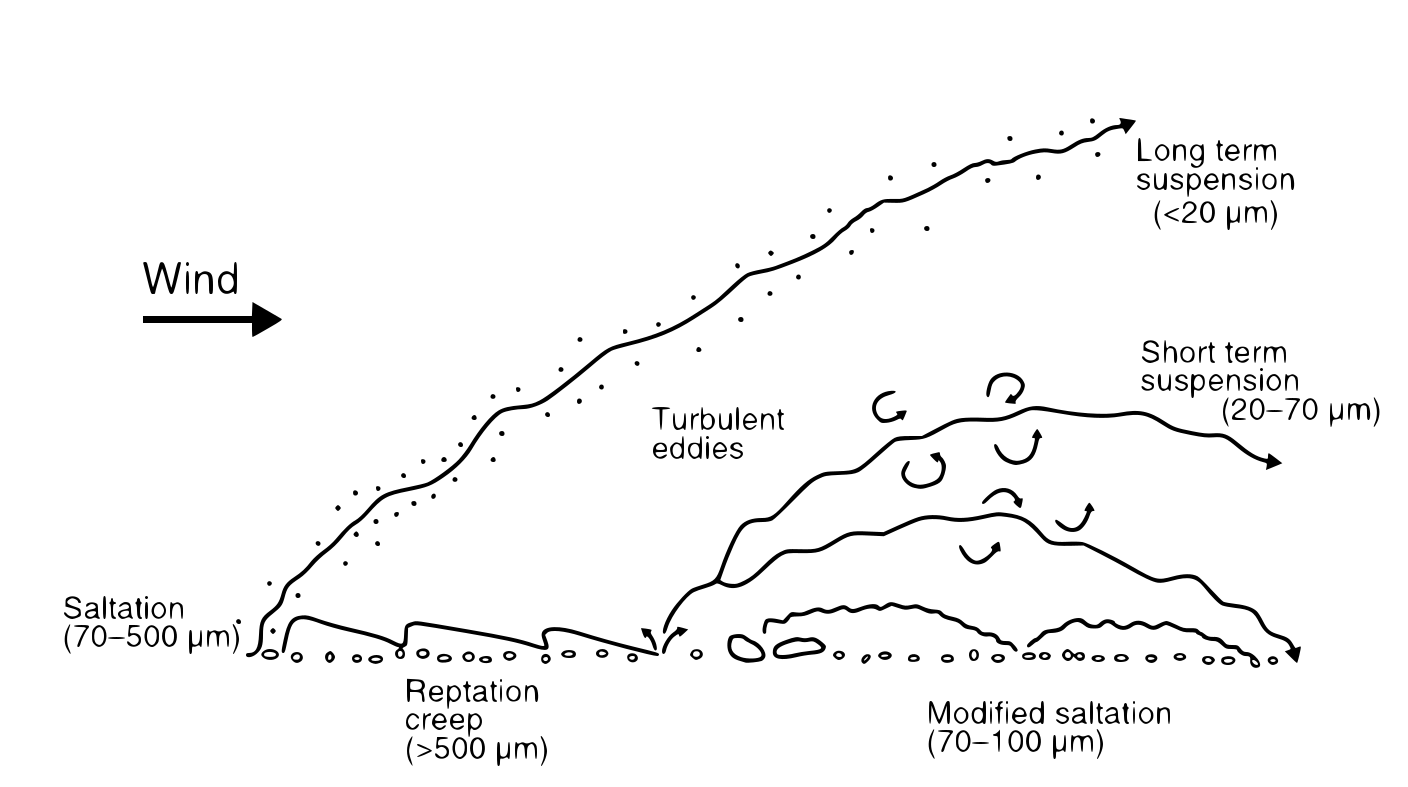
\includegraphics[draft=false,width = \textwidth]{texfiles/figs/aeolian_transport_Parsons_Abrahams.pdf}
  \caption{Different regimes of aeolian transport \parencite{nickling2009aeolian}}
  \label{fig:modes_of_dust_transport}
\end{figure}

Part of the reason why coarse dust is not well represented in current dust models is that they typically are non-spherical. Non-sphericity can have a significant impact on the settling velocity of the particle due to increased aerodynamic drag. The effect of the non-sphericity on settling velocity of dust particles was investigated by \textcite{mallios2020effects}, and they found that non-spherical dust particles could remain significantly longer in the atmosphere compared to spherical particles of equivalent particle diameter. The non-sphericity of dust particles is not included in current dust models. Moreover, dust models cannot directly model the turbulent properties of the near-surface flow. The surface turbulence is important for the entrainment of coarse dust \parencite{klose2013large} and in facilitating the dust to stay aloft longer \parencite{ryder2013impact}. Electric charging of the dust particles counteracting the gravitational settling has also been proposed to affect the lifetime of the dust particles and is something that remains to be explored in dust models.     

The transport of atmospheric dust can either be simulated in a Lagrangian or Eulerian framework. In the Lagrangian framework, the dust is treated as a discrete entity represented by many computational particles. The computational particles are suspended with the flow, and their trajectories are determined by integrating the particle motion. The dust concentration rarely exceeds more than several grams per kilogram of air. Therefore, the presence of dust aerosols does not significantly impact the density and dynamics of the flow \parencite{zhuang2001compositions}. Consequently, the motion of the dust particles can be determined separately from fluid motion \parencite{ShaoYaping2008PaMo}. Lagrangian models rely on tracking many computational particles to obtain statistically robust results and can thus be computationally expensive. In eulerian models, the dust aerosols are assumed to behave like a fluid. Therefore, the dust concentration follows the same kind of advection and conservation equations as other scalars in the atmosphere. In an Eulerian dust model, the atmosphere is discretised into grid boxes on a computational grid with a certain resolution, and in each grid box, the model calculates the dust concentration. However, because of the limited resolution of the grid, Eulerian models often suffer from excessive numerical diffusion, which causes filament structure in the transport to be smoothed out \parencite{cassiani_offline_2016}. In contrast, Lagrangian models do not require a computational grid and can therefore better preserve such filament structures in the transport \parencite{cassiani_offline_2016}.         

\subsection{Dust Deposition}
Dust can be removed from the atmosphere either through dry- or wet deposition. 
Dry deposition typically is the dominant process close to the source region as there are still many large dust particles present that fall out quickly. 
As the dust is transported further away from the source region, the larger particles fall out, and the dust size spectrum becomes narrower and the mode finer \parencite{does2016particle}.
Dry deposition becomes less efficient at finer particle sizes, and thus far from the source, wet deposition is usually the dominating process \todo{citation}.
There are two distinct routes a dust particle can be wet deposited, in-cloud or below-cloud scavenging: 
In-cloud scavenging, the dust particles are rained out from the cloud through serving as \acrshort{ccn}s or \acrshort{in}s or by colliding with existing cloud particles. Below-cloud scavenging involves the dust particles being captured by falling hydrometeors. 

In dust models, the deposition is typically represented by a deposition velocity. For dry deposition, the predominant factors deciding the deposition velocity are the dust particle size and the density. A multi-layer resistance scheme is commonly used in dust models to estimate the dry deposition rate. A widely used scheme used for modelling dry deposition is the two-layer resistance model of \parencite{slinn1982predictions}. The resistance model divides the atmosphere into two distinct layers; The quasi-laminar sublayer close to the ground, which has a thickness on the order of centimetres and the constant flux layer above. In the quasi-laminar sublayer, Brownian diffusion and gravitational settling are the two main deposition processes. Within the constant flux layer, turbulent motions and gravitational settling dominate. The gravitational settling velocity can be expressed by the modified stokes law of \parencite{slinn1982predictions}: 
\begin{equation}
    v_g = \frac{g\rho_p d_p^2 C_{cun}}{18\mu}
\end{equation}
Where $\rho_p$ and $d_p$ is the particle density and diameter, $\mu$ is the dynamic viscosity of air and $C_{cun}$ is the Cunningham slip-flow correction. The slip-flow correction accounts for the reduction in the drag force experienced by the smallest particles of sizes comparable to the mean free path of the molecules in air. The dry deposition velocity of a particle with a given size is given by a set of resistances, added to the settling velocity $v_g$:
\begin{equation}\label{eq:drydep_resistance}
    v_d=[r_a + r_b + r_a r_b v_g]^{-1} + v_g
\end{equation}
Here the $r_a$ represent the aerodynamic resistance, operating the constant flux layer, and $r_b$ represent the resistance in the quasi-laminar surface layer. There have been relatively few theoretical developments since the work of \textcite{slinn1982predictions} even though this model has been shown to reproduce the dependence of $v_d$ on particle size \todo{reference}, it does not differentiate the deposition velocity between different surfaces \parencite{shao2011dust}. The difference in deposition rate between different surfaces is expected to be quite large \todo{reference}. 

Many of the mechanisms involved in wet deposition are complex and generally not well understood\todo{citation} and some dust models do not consider wet deposition at all \parencite{zhang2019parameterization}. Between below-cloud and in-cloud scavenging, below-cloud scavenging is the simpler and better-studied process.
There are two mechanisms that affect the efficiency of below-cloud scavenging: (1) fine dust particles with diameters less than \SI{2}{\micro\metre} tend to follow the streamlines and flow around the droplet, and (2) the dust particles might bounce off after colliding with the droplet. 
Accordingly, below-cloud scavenging is typically most efficient for the larger dust particles \parencite{jung2006intercomparison}.
Currently, data is lacking for determining the probability of retention during the collision with the droplet, hence this mechanism is not included in current dust deposition schemes \parencite{ShaoYaping2008PaMo}. Several schemes for estimating the below-cloud scavenging efficiency $\lambda$ of varying levels of complexity have been proposed. The more advanced schemes, e.g. \textcite{seinfeld1998atmospheric, ShaoYaping2008PaMo}, uses semi-empirical relations to explicitly calculate the collection efficiency $E(r,R)$ as a function of both the droplet and dust particle radius. However, these schemes require knowing droplet size distribution which is not always available in the model. Therefore empirical below cloud scavenging schemes that directly relate scavenging coefficient to the precipitation rate, e.g. \textcite{brandt2002modelling} have been developed. These schemes avoid uncertainties in determining the collection efficiency \parencite{jung2006intercomparison}. Some empirical schemes, e.g. \textcite{laakso2003ultrafine} also includes a dependence of dust particle size for the scavenging efficiency. 
\begin{figure}[htpb]
    \centering
    \includegraphics[draft=False,scale=.5]{texfiles/figs/Scavenging.PNG}
    \caption{Comparison of below cloud scavenging coefficients for three different below-cloud scavenging schemes; $\lambda_1$ \textcite{jung2006intercomparison},$\lambda_2$ \textcite{brandt2002modelling} and $\lambda_3$ \textcite{laakso2003ultrafine}. Adopted from \textcite{jung2006intercomparison}}.
    \label{fig:scavenging}
\end{figure}
A comparison of the semi-empirical \textcite{ShaoYaping2008PaMo} scheme and empirical \textcite{brandt2002modelling} and \textcite{laakso2003ultrafine} are shown in \Cref{fig:scavenging}. For all the schemes, $\lambda$ increases for larger precipitation rates. Moreover, in the two schemes where $\lambda$ depends on the size of the dust particle, the scavenging coefficient decreases towards the \SI{1}{\micro\metre} mark and then increase again for the dust particles larger than \SI{2}{\micro\metre}.

Present understanding of in-cloud processing and especially for dust aerosols is lacking. Thus the representation of in-cloud removal of dust in models remains crude. Some dust models represent the dust as purely hydrophobic and neglect in-cloud scavenging entirely, while other models assume dust scavenging efficiency to be that of sulphate \parencite{bergametti2014dust}. Yet a realistic representation of the wet removal process is crucial for  

% \subsection{Dust Observation}
% Dust observations are crucial for advancing current dust models. The advent of earth-observing satellites has helped to constrain the location of the dust sources.    

\section{East Asian Dust}
The East Asian region has a long-lasting history of aridity. The oldest evidence of aridification in this region dates back to the late Oligocene \parencite{qiang2011new}. Since the Miocene, global cooling and combined with the uplift of the Tibetan Plateau have further expanded the arid environment of Northern East Asia \parencite{miao2012controlled}.  
The focus of this thesis is the East Asian dust sources and how the dust gets transported and deposited over the \acrshort{clp}. Conversely, this section will introduce the study area and describe the spatial and temporal variations of dust emissions in this region.  

\subsection{Spatial Distribution and Characteristics of Dust Sources and Area Regions}\label{sec:spatial_temporal_dust}
The majority of the East Asian deserts are located in the Northern part of China and South East Mongolia, as shown in \Cref{fig:maps_clp_deserts}b. The precipitation patterns predominately determine the distribution of the deserts.
Situated in the interior of the Eurasian continent, the deserts are far removed from the moisture of the Pacific Ocean. 
The dry conditions are exacerbated by the Tibetan Plateau and the Himalayas, inhibiting the transport of air masses from the southwest.  
In total, the East Asian deserts make up the second-largest source of atmospheric dust on the planet with an approximate annual dust emissions of 2000 Mt \parencite{chen2017overview}. 

\begin{figure}[htpb]
    \begin{subfigure}[b]{0.38\textwidth}
        \centering
        \includegraphics[width=\textwidth]{texfiles/figs/map_loess.pdf}
        \label{fig:map_clp_locations}
        \caption{}
    \end{subfigure}
    \hfill
    \begin{subfigure}[b]{0.58\textwidth}
        \centering
        \includegraphics[width=\textwidth]{texfiles/figs/map_sources_china.png}
        \label{fig:map_deserts}
        \caption{}
    \end{subfigure}
    
    \caption{Map of the \acrshort{clp} (a) with the prominent loess sites marked. (b) The major deserts in East Asia, with the mobile sands, semi-mobile sands and Gobi regions areas indicated, modified from \textcite{mao2013numerical}. }
    \label{fig:maps_clp_deserts}
\end{figure}

In terms of the morphology and composition of the surface soil, the East Asian deserts can be separated into two classes gobi-deserts and sand deserts \parencite{xuan2002characterization}. The Gobi is characterised by regions consisting of pebbles, gravel and rock debris. Accordingly, the Gobi desert refers to an area consisting of interluding regions of sandy deserts, gobies and grasslands.
Gobies and the Gobi desert mainly cover the northern region of the Inner Mongolia Plateau and the southern part of Mongolia (\Cref{fig:maps_clp_deserts}b). \todo{add some more info on Gobi}

This region also fosters many sand deserts that mainly consists of loose sand. The loose sand facilitates dune formation, and the worlds tallest dunes are situated in the Badain Jaran desert. 
The dunes are so large that they can generate their own weather \parencite{dong2013investigation}. The most significant sand desert in the region is the Taklamakan desert, located in the Tarim Basin. 
The Tarim Basin is extremely dry, with annual precipitation of as low as 20mm. The extreme dryness makes it impossible for vegetation to set root, conversely the region has a very small threshold friction velocity of about 4 m/s compared to 7 m/s for the Gobi desert \parencite{ShaoYaping2008PaMo}. Therefore, the Taklamakan experience the highest number of days with blowing sand among the East Asian deserts. However, the desert is well shielded from the weather by mountain ranges on all sides except for the opening at the eastern side of the basin, therefore dust storms less frequent \parencite{ShaoYaping2008PaMo}. 

There are also several deserts located in close proximity of \acrshort{clp}. Among the larger deserts being the Tegger desert, Ulan Buh desert and Mu Us desert. 

\subsubsection{The Chinese Loess Plateau}
A large portion of the dust emitted from the desert in East Asia gets transported and deposited over the \acrshort{clp}. 
The thickness of the loess deposits on the \acrshort{clp} varies from 10 meters to several hundred meters. 
The spatial variation in the thickness of the Loess is part of what makes the \acrshort{clp} such a valuable environmental record. \todo{why?} The Chinese loess record consists of two main sequences: The Quaternary sequence, which consists of alternating layers of paleosols and loess that spans the entire Quaternary extending into the Pleistocene \parencite{maher2016palaeoclimatic}. The alternating paleosol and loess layers indicate the inter-glacial and glacial periods.  Underlying the Quaternary sequence is the Red Clay formation which is of similar aeolian origin and extend the loess record into the Miocene. In contrast to the Quaternary sequence, the Red Clay sequences are continuous without interluding paleosol layers. This means that the Red Clay was formed under relative humid conditions in contrast to the colder climate during the Quaternary \parencite{yang2004comparison}. 

The locations shown in \Cref{fig:maps_clp_deserts}a are all prominent Loess sites. The spatial variation in the provenance of the \acrshort{clp} loess has been investigated both for the Quaternary, Red Clay sequence and present day\parencite{shang2016variations}. \textcite{shang2016variations} investigated the spatial variation in the provenance of the Red Clay, where they found that the southern \acrshort{clp}  (Lingtai, Lantian and Luochuan) had U-Pb age distributions similar to that of the northern Tibetan Plateau and Taklamakan compared to eastern \acrshort{clp} (Baode) which in addition had a peak at 200-300 similar to the age distribution. 
\begin{itemize}
    \item The \textcite{sun2003seasonal} can be informative here
    \item Red Clay vs Quaternary Loess
    
\end{itemize}
%On the Loess Plateau, the content of silt and clay in the surface soil is more than 90\% and the sand and gravel content is in totally lacking (Xiong and Li, 1990). Also, the annual mean precipitation is around 400 mm yr

%Loess Plateau is the center of a strong dust-fall region. Their chemical analysis of soil samples proves also that the Loess Plateau was formed by millions of years of dust deposition (Zhang, 1999).


\subsection{Meteorological conditions of dust storms}
In East Asia the around 80\% of the dust events occurs in spring months from March until May, with half of the dust events occurring in April \parencite{sun2001spatial}. The occurrence of dust events are strongly correlated with the surface wind speed \parencite{kurosaki2003recent}. Strong surface wind speeds are typically generated by passing cold fronts and synoptic scale cyclones associated with cold air outbreaks \parencite{sun2001spatial, zhou2003typical, takemi2005dust}.
Moreover cold fronts promotes strong and deep vertical mixing due to the strong surface heat flux in the cold frontal regions. The deep mixed layer can carry the dust into the upper troposphere allowing the dust to be transported far downwind \parencite{liu2003high}. 
  
Dust storms in Gobi desert and the desert regions north west of the \acrshort{clp} are usually due to the development of deep low pressure system over Mongolia. Cold air outbreaks producing dust event in this region typically follow a northerly path, passing near lake Baikal and the moving southward across across southern Mongolia and China.     


\begin{itemize}

    \item Cold wave outbreaks
    \item Mongolia Cyclone
\end{itemize}
In the winter, the desert regions are dominated by the cold \acrshort{sh} causing parts of the desert to be covered in snow and the soil to frozen. The frozen soil thaws in spring, leaving the surface loose and prone to wind erosion. 
The majority of the dust events in East Asia occur during the spring months from March until May, with half of the dust events occurring in April \parencite{sun2001spatial}. The dust storms are associated with cold air outbreaks, which initiate the formation of the Mongolian cyclone and frontal systems. About 80 \% of the dust events are associated with an active Mongolian cyclone, whereas the remaining are caused by the passage of cold fronts \parencite{sun2001spatial}.
The number of cold air outbreaks occurring in spring is much influenced by the intensity and location of the jet stream. A strong jet stream inhibits air mass exchange between lower and higher latitudes whereas and confine the cold air to the high latitudes \parencite{wang2008variability}. There has been a large decrease in the number of dust events in East Asia since the 1980s, which has been hypothesised to be the result of arctic amplification and weakened temperature gradients \parencite{liu2020impact}. 

\subsection{Influence of Regional and Large-scale Climatic Factors on Dust Deposition to \acrshort{clp}}
The most prominent feature of the atmospheric circulation in the East Asian region is the monsoon system. A monsoon system seasonally changes wind direction, blowing from one direction in the summer and the opposite direction in the winter. The primary driver of the East Asian monsoon system is the temperature contrast between the land and ocean. During the winter months, the land is generally colder than the ocean, with the main heating source located over the equatorial western pacific. The convection associated with the heating drives a large scale meridional overturning circulation where the airmasses rise over the ocean and then subsides over the Siberian region. Creating a persistent high-pressure system over Siberia during the winter. This circulation is the East Asian Winter Monsoon (EAWM). During the East Asian Summer Monsoon (EASM) the situation is reversed. In the summer, the land is much warmer than the ocean, and the heating on land drives strong convection, which creates a persistent low pressure at the surface. The low pressure drags moist air from the ocean inland. Upon reaching the Tibetan Plateau, the moist air is lifted and consequently cooled, which causes the water vapour to condense, resulting in intense precipitation. 

\emph{I think this section should start with descrbing the summer monsoon and then move on the winter monsoon.}

%\subsubsection{East Asian Winter Monsoon}
\begin{figure}[htpb]
    \centering
    \includegraphics[width=\textwidth]{texfiles/figs/climatology_1999-2019.pdf}
    \caption{The 20 year average of winter (DJF)  and spring (MAM) circulation from ERA5. (a) Winter and (b) spring \acrshort{mslp} and 850hPa winds climatology. (c) Winter and (b) spring 500hPa geopotential height and winds. (e) winter and (f) spring 200hPa geopotential height and wind speed.}
    \label{fig:clim_circulation}
\end{figure}
%The EAWM dominates the climate in East Asia during the winter months, December, January, February, and is closely related to the cold-core of the Siberian High. The \acrshort{eawm} circulation is primarily driven by the temperature contrast between the relative cold and warm ocean. \acrshort{eawm} consists of 3 subcomponents which can be identified in \Cref{fig:clim_circulation}, at the surface the Siberian High and Aleutian low, East Asian trough can be identified at the 500hPa level located around 120\degree E and 50\degree N  
\begin{figure}[htpb]
    \centering
    \includegraphics[width=\textwidth]{texfiles/figs/winter_MO_AO_composite.pdf}
    \caption{Circulation composite anomalies of 850hPa winds and mean sea level pressure for strong - weak winter monsoon years and negative - positive winter AO. (a) and (b) is the DJF anomalies and (c) - (d) is MAM anomilies in the following spring}
    \label{fig:mo_ao_composite}
\end{figure}

\subsubsection{The impact of Arctic Oscillation on the East Asian climate}
\begin{figure}[htpb]
    \centering
    \includegraphics[width=\textwidth]{texfiles/figs/EOF_AO_NAO.pdf}
    \caption{The spatial correlation of the leading EOF of 1000hPa geopotential height (a) representing the \acrshort{ao}. (b)  spatial correlation of the leading \acrshort{eof}  of SLP anomalies over the Atlantic sector, 20\degree-80\degree N, 90\degree W-40\degree, representing the \acrshort{nao}.}
    \label{fig:EOF_NAO_AO}
\end{figure}
The \acrfull{ao} is represented by the leading EOF of the 1000hPa geopotential height poleward of 20 \degree N \parencite{thompson1998arctic}. In its structure, it resembles the \acrfull{nao} except being more zonally symmetric in structure. The AO has been shown to have a significant impact on the \acrshort{eawm} where negative winter AO is usually associated with a stronger winter monsoon and vice versa. Cold events are also found to be more frequent over East Asia during negative AO conditions \parencite{he2017impact}. \textcite{wu2002winter} examined how the \acrshort{ao} influence the \acrshort{eawm} and found that the AO directly influence surface air temperature (SAT), \acrshort{mslp} and the East Asian Trough at 500 hPa over the region northwards of 35°N in East Asia rather than through its impact on the SH. The SH, in comparison, has a more direct impact on the \acrshort{eawm} through influencing the \acrshort{mslp} and the northerly wind along the East Asian coast. However, due to the how \acrshort{ao} suppresses the influence of the \acrshort{sh} on the higher latitudes, the influence of the \acrshort{sh} happens primarily southwards of 50\degree N over East Asia \parencite{wu2002winter}. 

\begin{figure}[htbp]
    \centering
    \includegraphics[width=\textwidth]{texfiles/figs/winter_MO_AO_composite_500h.pdf}
    \caption{Circulation composite anomalies of 500hPa winds and geopotential height for strong - weak winter monsoon years and negative - positive winter AO. (a) and (b) is the DJF anomalies and (c) - (d) is MAM anomilies in the following spring}
    \label{fig:mo_ao_composite_500hPa}
\end{figure}






% it has been known that there are three major motions of wind‐blown sand particles, i.e., creep, saltation, and suspension

% Except for dust storms in which the suspension motion is dominant, saltation plays a key role in the wind erosion process


%And, southwest of the plateau, the bottom of the Old Tarim Basin and Old Junggar Basin had also lifted to 1000 m elevation but still remained lower than the surrounding topography. The modern Tarim Basin and Junggar Basin are surrounded by the Altaj Mountains in the north, Tainshan Mountains in between, Tibetan Plateau in the south, Pumir Plateau in the west, and Mongolian Plateau and Kunlun Mountains in the east

%It is suggested that the source region in East Asia consists of two parts or systems: (i) the Mongolian Plateau dust source system, including deserts and gobi-deserts on the Mongolian Plateau and its southern extension—the Ordos Plateau and Alxa Plateau; and (ii) the Tarim Basin dust source system, including deserts and gobi-deserts in the Tarim Basin, Junggar Basin, and eastern vicinity.

%classified dust storms in East Asia into four types, among which the S (stationary) type and M (moving) type are basic ones. 80\% of their S type dust storms occurred over the Taklimakan Desert and vicinity, while 70\% of the M type originated over the gobi area and desert area of 90–105°E, i.e., the Mongolian Plateau and its southern extension.


%Gravel covering the gobi surface can effect the dust emission both positively and negatively: gravel half-buried in sand (soil) surfaces decreases the effective wind shear force on the soil surface, resulting in stress partitioning (Nickling and Gillies, 2003), and a complete stony armor strongly depresses the aeolian motion of particles (Yi et al., 2002). 

%precipitation is rare in the gobi area, less than 50 mm yr−1 (Zhao, 1994), and is limited to the summer season so that the gobi surface becomes extremely dry in spring when the strong wind behind a cold front periodically blows through East Asia and is enhanced over the vast and flat gobi surface. As the surface wind speed often reaches 24–30 m s−1, or even higher, on the south Mongolian Plateau (Qian et al., 1997), strong dust storms occur in spite of the gravel armoring and the below 0°C air temperature. 

%Thousands of kilometers from the oceans and high above the sea level, the Mongolian climate is extremely dry, continental and cold.

%  It is also normal in Mongolia that the annual precipitation varies greatly from year to year. For example, the precipitation in Sainshand (44°52′N, 110°09′E) was 83 mm yr−1 in 1963 but, in the next year, it went up to 248 mm yr−1 (CMA, 1970). Such a great interannual change in precipitation means that, in drought years, severe dust storms occur even in the north mountain area. At the end of winter season, the south Siberian anti-cyclone named the ‘Siberian High’ becomes unstable and, in the following spring months, breaks down several times so that a succession of frontal systems traverses the country from northwest to southeast, resulting in strong surface wind, which is further strengthened over the vast and flat gobi surface. 

%In the Mongolian Plateau system and downwind vicinity, from northwest to southeast, the surface soil texture shows a coarse-to-fine trend: gobi gravel becomes desert sand, followed by silt and clay of the Loess Plateau. 

%A cold front passage in spring produces strong surface wind in both systems. Because of the difference in topography, northwest wind and northeast wind respectively prevail in the Mongolian Plateau system and the Tarim Basin system. 

